\documentclass[a4paper, 11pt]{article}
\usepackage{graphbox}
\usepackage{fancyhdr}
\usepackage{caption}
\usepackage{fancyvrb}
\usepackage{float}
\usepackage{pgfgantt}
\usepackage{textcomp}
\usepackage{etoolbox}
\patchcmd{\thebibliography}{\section*{\refname}}{}{}{}

\fancypagestyle{title}{
\renewcommand{\headrulewidth}{0pt}
\fancyhf{}
\lhead{Luke Bessant - 2019}
\rhead{}
}
\pagestyle{title}

\title{\textbf{CS3821 Full Unit Project}\\Interim Report of Progress}
\author{Luke Bessant\\Supervisor: Reuben Rowe}
\date{\today}

\begin{document}

\maketitle
\thispagestyle{title}
\newpage

\tableofcontents
\clearpage
\newpage

%%%%%%
\part{Review}
\section{The Project So Far}
Since the beginning of this project a surprising amount of work has been put into both research into the theory surrounding the key aspects of the subject, and the implementation of such theory in proof of concept programs. Steady progress has been made towards the final objective of the project, being a compiler for a subset of the Java programming language, with each program and report written building the knowledge necessary to complete said objective in the next term.

\subsection{Deliverables}
I would say that the overall progress of the project thus far has been very good, with the deadlines I set for myself being met in most cases. It is only in the last few weeks that reports have been escaping deadlines due to a heavy concentration on implementation of the lexer generator program later detailed. Therefore a reflection on this point for future consideration would be to muster the discipline necessary to work on writing reports as well as programming.
\\\newline
In terms of programs written, all of the deadlines were met with much time to spare, allowing me to move onto subsequent programs, sparing time which later allowed me to add the lexer generator program to the project. In hindsight I would say that I overestimated the time it would take to complete the first two programs, the BNF pretty printer and the calculator interpreter. If I had started these easlier I would have been able to fit in a fourth proof of concept program perhaps on parsing.

\section{Continuation}
\subsection{Aims and Objectives}
The key aim for the second term of the project is to create a working compiler for a subset of the Java programming language most notably including control flow, use of memory, arithmetic and decision making. On top of these other support including that of methods and classes could be constructed if progress is better than expected.
\\\newline
Secondly, a final report will be written on the overall progress of the project spanning the two terms. This will include detailed information on the inner-workings of the compiler deliverable and a reflection on how the project has played out over the academic year.
\\\newline
The main objective of the project from this point is to make a stable working compiler which can take in code written by the user in the language to be specified, and generate the corresponding low level executable representing program written by the user.

\subsection{Continuation gantt chart}
The gantt chart below shows the planned time-scale of the individual project split into weeks one through twelve for the second term of the academic year. \\
\begin{center}
	\begin{ganttchart}[
		vgrid,
		group/.append style={draw=black, fill=black!25},
		milestone/.append style={shape=star}]{1}{12}
	\gantttitle{Term 2}{12} \\
	\gantttitlelist{1,...,12}{1}\\
	\ganttbar{Final Program (27/03/20)}{1}{10} \\
	\ganttmilestone{Final Report Draft (28/02/20)}{8} \\
	\ganttbar{Final Report (27/03/20)}{4}{12} \\
	\ganttmilestone{Final Programs/Report (27/03/20)}{12}
	\end{ganttchart}
\end{center}

\noindent The large expanse of time allocated to both the final program and report should allow sufficient time to carry out the research and implementation necessary to complete the project in good time.

\clearpage

%%%%%%


\part{Research}
\setcounter{section}{0}
\section{Interpretation}
One of the significant means of correctly executing a program written in some language is to employ an interpreter. Considering the importance of interpreters and the proposed implementation of a simple four function calculator for this project to prove the concepts of lexing, parsing and evaluation, the purpose of this section is to represent how interpreters work and aid me in constructing one.

\subsection{Interpreters}
Simply put an interpreter is a program designed to execute code written in some language by taking the code file or stream as input, and produce the desired output of said code rather than an executable program. This is done by traversing the lines of code in the input program consecutively, processing each line individually and generating their outputs one-by-one, not taking into account the larger code block around it. Thus a given line is more or less independent from those around it, other than sharing access to the same stack frame when within the same procedure, thereby having access to the variables and data models made available to other lines of code of that procedure.
\\\newline
Considering this procedure of running each line of a program one after the other, it can be derived that particular lines will be run more than once within certain programs. For instance the presence of a loop mandates that the code block within the loop will be run as many times as it takes until the loop terminates. This is a key inefficiency concerning interpreters and one of the reasons that interpretation is generally slower than compilation. The \textit{executable} we use to begin the running of a program written in an interpreted language is the interpreter itself, to which we pass our plaintext code.
\\\newline
Some examples of interpreted languages include Bash, VBScript and MATLAB. It's common that widely used languages will compile source code into an intermediate code or bytecode, which they then interpret. Languages fitting this description include Java and Python.

\subsection{The Process of Interpretation}
This first step performing lexical analysis on the plaintext representation of the input code, written in the high level language supplied by the programmer and understood by the interpreter. The process of lexical analysis is to split the source code into a list of tokens, in other words, to \textit{tokenise} the code. This process of lexical analysis will be detailed in the next section of this report. The stream of tokens is then passed to the syntax analysis phase, detailed in section 4, which generates an \textit{abstract snytax tree}.
\\\newline
Following its generation the abstract syntax tree is passed to an evaluator in a structured list form, whose task is to process this list in such a way that the desired output result of the original code passed to the lexer is produced. This could be done by recursively evaluating each branch of a given tree node, perhaps the left side of the operand within a simple addition expression and then the right, and then evaluating the addition itself using the remaining left and right leaves.

\subsection{Interpretation vs. Compilation}
The processes of interpretation and compilation are structurally near-identical until the aforementioned evaluation stage after the generation of an abstract syntax tree. At this point, the interpreter goes on to directly evaluate the statements held within the tree and execute them to produce an immediate output. This makes interpreted programs easier to debug as we would be evaluating a particular line when an error occurs. Contrastingly a compiler will, from the AST, generate intermediate code in some low level language which is platform-independent. A good example of this would be the compilation process for C.
\\\newline
Therefore an interpreted program will usually begin execution more quickly than a program needing compilation, however due to the optimisation and code generation steps used by a compiler, the compiled program will generally be faster when running the executable file it generates. In addition, this executable will always be ready to run. An interpreted language requires the presence of an interpreter program to execute programs written using it, whereas only the executable file generated by the compiler is necessary for a given platform.
\\\newline
Since an interpreter relies on the presence of a plaintext source code file in its specified language, code written in an interpreted language will always have openly readable source code, unlike a compiled program consisting of byte code. Therefore we are able to keep the source code more private when using a compiled language.

%%%%%%

\clearpage
\section{Context-Free Grammar Specifications}
A context-free grammar is a language specification which allows a computer to derive the desired grammatical structure intended by the programmer to a list of tokens, from the lexical analysis phase, which make up a statement. This gives a computer the ability to understand its meaning and therefore generate the correct syntax tree for the statement which is then used in later stages of compilation or interpretation. Take for instance the following:

\begin{center}
	\textit{statement} \textbf{\textrightarrow} \texttt{while}(\textit{expression})\texttt{:} \textit{statement}
\end{center}

\noindent Represented here is a production rule for a \textit{statement}, in this example a while loop. The string on the right side is a concatenation of the keyword \textbf{while}, an opening parenthesis, a nonterminal \textit{expression}, a closing bracket, a colon, and a nonterminal \textit{statement}. We can add in the below two production rules to our grammar and assign the nonterminal 'statement' as the start symbol.

\begin{center}
	\begin{tabular}{l}
		\textit{expression} \textbf{\textrightarrow} \texttt{True} \\
		\textit{statement} \textbf{\textrightarrow} \texttt{print(}\textit{expression}\texttt{)}
	\end{tabular}
\end{center}

To allow us to generate the below string \texttt{while(True): print(True)}, belonging to the language generated by this grammar using nonterminals and terminals. \textit{Nonterminals}, terminals and production rules will be outlined in the following subsection.

\subsection{Specification}
A correctly specified context-free grammar must consist of the following components:

\begin{itemize}
	\item A set of \textit{terminal} symbols. These are characters or keywords which make up the strings of the language, e.g. \textit{[a..z]}, \textit{[0..9]} or mathematical operators. These make up the \textit{alphabet} of the language generated.

	\item A set of \textit{nonterminals} which represent the strings we can derive using their production rules. Each is the head of at least one production rule, describing the strings that can be derived from it.

	\item A list of construction rules known as \textit{productions}, defining the strings that can be created from a nonterminal. A nonterminal is \textit{head} (left side) of the production, separated by the symbol \textbf{\textrightarrow} or \textbf{::=} as ``has the form", from the \textit{body} of the production (right side), consisting of a pattern of terminals and nonterminals.

	\item Identification of the \textit{start symbol}, a nonterminal, usually the first listed or otherwise designated visually, from which we can derive all of the strings which make up the language generated by the grammar.
\end{itemize}

\subsubsection{Example}
An example for a simple two function calculator context-free grammar specification is shown below:

\begin{center}
	\begin{tabular}{l}
		\textit{operand} \textbf{\textrightarrow} \textit{operand}\texttt{+}\textit{operand} \\
		\textit{operand} \textbf{\textrightarrow} \textit{operand}\texttt{-}\textit{operand} \\
		\textit{operand} \textbf{\textrightarrow} \texttt{a}
	\end{tabular}
\end{center}

The terminals \texttt{a, -} and \texttt{+} are shown in bold, and the nonterminals are italicised. To note, we can use the ``\textbar"\ symbol to combine multiple productions with the same head into one production as below:

\begin{center}
	\begin{tabular}{l}
		\textit{operand} \textbf{\textrightarrow} \textit{operand}\texttt{+}\textit{operand} \textbar\ \textit{operand}\texttt{-}\textit{operand} \textbar\ \texttt{a}
	\end{tabular}
\end{center}

Some examples of the strings contained within the language generated by this grammar are \texttt{a, a+a, a+a-a} and \texttt{a+a+a+a}. 

\subsection{Derivations}
We \textit{derive} strings belonging to the language of a grammar by beginning with the start symbol and replacing the nonterminals its body with the body of a production for that nonterminal, eventually ending up with a string which is an element of the language. For the grammar specified in Section 3.1 with the start symbol being our only nonterminal, \textit{operand}, we can replace this symbol with \textit{operand}\texttt{+}\textit{operand}, \textit{operand}\texttt{-}\textit{operand} or \texttt{a}.
\\\\
We show that a nonterminal $\alpha$ \textit{derives} a terminal or other nonterminal $\beta$ by $\alpha \Rightarrow \beta$. This is also called a replacement. We can show the derivation of a particular string by replacements. For example:

\begin{center}
	$operand \Rightarrow operand+operand$ $\Rightarrow \texttt{a}+operand$ $\Rightarrow \texttt{a+a}$
\end{center}

This shows the \textit{derivation} of \texttt{a+a} from \textit{operand}, proving that \texttt{a+a} is a string of the grammar from Section 3.1. During parsing we take a string of terminal symbols such as the one shown above and then try to figure out how to derive it from the start symbol.

\subsection{Backus–Naur Form Notation}
Backus–Naur form or BNF for short is simply a language for creating context-free grammar specifications, thus such specifications have near-identical structure to the previous examples of context-free grammars. Every rule in BNF takes the form:

\begin{center}
	\begin{tabular}{l}
		\textit{head} \texttt{::=} \textit{body}
	\end{tabular}
\end{center}

\noindent We can define the grammar previously defined in BNF with the following:

\begin{center}
	\texttt{operand ::= operand '+' operand \textbar\ operand '-' operand \textbar\ 'a' .}
\end{center}

\noindent The example shown above also defines a \textit{recursive statement} since the production rule makes use of the head nonterminal in its body. We can also surround certain contents of the body of a BNF production in curly braces to indicate zero or more repetitions of the contents. For example, when specifying functions which take a list of parameters we can use \texttt{\{<parameter>\}} within the body to indicate zero or more parameters. In conclusion, the use of BNF is to give us a standard syntactic structure for specifying context-free grammars.

%%%%%%

\clearpage
\section{Lexical Analysis}
As the first stage in the compiler toolchain, lexical analysis takes the raw source code of a program written in a language supported by the compiler and processes it in such a way that the program is split up into \textit{lexemes}, which by their character pattern are identified as particular \textit{tokens}, and then passed to the parser for syntax analysis. Lexemes are sequences of characters which match the pattern for a particular component of the programming language supported by the compiler. These lexemes represent the individual parts which make up a statement or expression within a program. Take the expression below:

\begin{center}
	\texttt{sum = sum + 50}
\end{center}

\noindent We can split this expression into the lexemes \texttt{sum}, \texttt{=}, \texttt{sum}, \texttt{+} and \texttt{50}, and are able to tell that this simply adds 50 to the current value of \texttt{sum} and reassigns the result as \texttt{sum}. Since the lexical analyser simply takes the stream of characters from our source program, it has to create lexemes from a sequence of consecutive characters using the production rules for tokens outlined within the grammar for the language. This stream of tokens is then sent to the next stage, syntax analysis to be structured.

\subsection{Tokens}
A token is a pair of the form \textlangle{}\textit{token-name, token-attribute}\textrangle{} denoting the type and contents of a valid lexeme. Many lexemes can match the pattern for a token, therefore we have the option to use an attribute for the token to give the compiler more information about it. This could be a literal value or a pointer to a position in the program's \textit{symbol table}. Upon discovering a pattern matching a valid token, the lexeme is identified by the lexical analyser as an instance of that token. 
\\\newline
For example, the lexeme \texttt{50} in the above expression could be recognised as an \texttt{integer} token and thus the lexer will create the token \textlangle{}\texttt{integer, 50}\textrangle{}. The lexeme \texttt{sum} could match the pattern of an \textit{identifier}, in which case a possible token could take the form \textlangle{}\texttt{id, 1}\textrangle{}. Here \texttt{id} is shorthand for identifier, and \texttt{1} is a pointer to a location within the program's symbol table where more information about the identifier is held, such as the identifier's name, type and current value. Some of the common token types across programming languages are as follows:

\begin{itemize}
\item A token for all identifiers within the language.
\item A token for the keywords within a language, such as \texttt{if} and \texttt{else}.
\item One token all mathematical and boolean operators, or one for each individually.
\item Tokens for literal strings and types of numbers supported by the language.
\item Tokens for punctuation symbols such as brackets, commans and semi-colons.
\item A token for whitespace, which is usually not passed to syntax analysis but is instead omitted by the lexer.
\end{itemize}

\subsubsection{Attributes of Tokens}
In cases where many lexemes match the pattern of a token, we need to pass more information about the lexeme to the parser so the correct incantation can be properly reproduced in the code generation phase of the toolchain. The name/type of the token is used within the parser to make decisions about program structure, whereas the attribute value is used later on when translating tokens during code generation. From the above example, we have \textlangle{}\texttt{integer, 50}\textrangle{}.
\\\newline
For the identifiers of a program we need to encompass several pieces of information within one token, such as the name, type and current value of the identifier. In these cases the token attribute would point to an entry in the program symbol table where this information is held. As we saw from the previous section, an example of this is \textlangle{}\texttt{id, 1}\textrangle{} where \texttt{1} represents row one within the symbol table.
\\\newline
For keywords and operations of which the raw characters of the lexeme match the token name, we can simply omit the attribute and use only the token name within the token. An example of this could be \texttt{if}, where we can discard the attribute value, which matches the token name, and simply use the token \textlangle{}\texttt{if}\textrangle{}.

\subsubsection{Recognition of Tokens}
Using finite-state automata we can model each of the production rules for the tokens of our grammar by converting their regular expression to a set of states with transitions between them, a transition for each of the potential letters the expression should recognise. For instance we have the following finite-state automata for a production \texttt{id} \textbf{\textrightarrow} \texttt{letter(letter|digit)*}:

\begin{figure}[H]
	\centering
	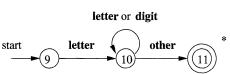
\includegraphics[width=60mm]{/home/luke/Pictures/FA.png}
	\caption{Finite-state automata for \texttt{id} (figure 3.14 from \textit{Aho - Compilers - Principles, Techniques, and Tools - page 132)} \label{overflow}}
\end{figure}


\noindent This accepts only patterns beginning with at least one letter, and then allowing any number of letters or numbers following this. If we read a character which is not a letter or digit, then we know that this is not part of the identifier comprised of the previous characters, so we can move to the accepting state. The asterisk atop the accepting state signifies that the last character of the lexeme (\textbf{other}) is not a valid member of the pattern for this token and so the \textit{forward pointer} of the scanner is retracted by one character so as to point to the last character of the identifier. We can determine that any sequence of characters leading to the accept state of this finite-state automata, except the \textbf{other} character, makes up an identifier as defined by our grammar.

%%%%%%

\clearpage
\section{Sentential Derivations and Top-down Parsing}
The syntax analysis phase within the compilation chain involves taking the stream of tokens derived from some source code using lexical analysis, and organising them into a syntax tree which represents the grammatical structure intended by the writer of the source code. This section will describe how to derive an input string belonging to the language of the grammar in use from its the start symbol, the construction of syntax trees from such derivations and the key aspects of the top-down parsing method.

\subsubsection{Syntax trees}
The syntax tree shown below, with accompanying grammar, gives an example tree structure for an expression \texttt{id + id * id}, where the operators are separate tokens with each \texttt{id} being an identifier.

\begin{figure}[ht!]
	\centering
	\includegraphics[width=90mm]{/home/luke/Pictures/grammar_example.png}
	{\caption*{(4.7): \textit{Aho - Compilers - Principles, Techniques, and Tools - page 222}} \label{overflow}}
\end{figure}

\begin{figure}[ht!]
	\centering
	\includegraphics[width=40mm]{/home/luke/Pictures/syntax_tree.png}
	{\caption*{Figure 4.5: \textit{Aho - Compilers - Principles, Techniques, and Tools - page 204}} 
	\label{overflow}}
\end{figure}

From this simple tree we can see that we must add to the leftmost \texttt{id} the result of the rightmost subtree of the root node (\texttt{id * id}), the start symbol of our grammar, \texttt{E}. Each inner node is is a production of our grammar and each leaf is either a terminal or nonterminal.

\subsection{Derivations}
The stream of tokens received from the lexer allows us to derive the structure of the tree corresponding to a clause, and the contents of the leaves by rewriting rules starting from the starting symbol (\texttt{E} in figure 4.5). Such rewriting involves taking some nonterminal and replacing it with the body of one of the productions for which that nonterminal is the head. By the grammar shown in (4.7), we can make the following derivation steps: 
\begin{center}
$\texttt{E} \Rightarrow \texttt{E+E} \Rightarrow \texttt{E+E*E} \Rightarrow \texttt{id+E*E} \Rightarrow \texttt{id+id*E} \Rightarrow \texttt{id+id*id}$
\end{center}
We say that \texttt{E} \textit{"derives"} \texttt{id+id*id}, proving that \texttt{id+id*id} belongs to the language generated by the grammar, that it is a \textit{sentence} of the language. Sentences which can be derived from the start symbol are \textit{sentential forms} of the grammar. If we can derive a string $\alpha$ from a start symbol \textit{S} in some sequence of zero or more derivation steps then $\alpha$ is a sentential form of the grammar.
\\\\
At each step in the derivation we have a choice of which nonterminal to replace, and which production with that nonterminal as a head to replace it with. A \textit{leftmost} derivation is one where we always pick the leftmost nonterminal of the current sentence to replace. The alternative is \textit{rightmost} derivation.

\subsubsection{Parse tree derivation}
Parse trees allow us to represent the grammatical structure of a sentence at any given step in the derivation sequence. Assume our current syntax tree consists of merely the start symbol \texttt{E}. By applying the derivation $\texttt{E} \Rightarrow \texttt{E+E}$ we simply add three child nodes to our current root node \texttt{E}; \texttt{E}, \texttt{+} and \texttt{E}, shown below.

\begin{figure}[ht!]
	\centering
	\includegraphics[align=c,width=16mm]{/home/luke/Pictures/syntax_tree2.png}
	$\Rightarrow$
	\includegraphics[align=c,width=30mm]{/home/luke/Pictures/syntax_tree3.png}
\end{figure}

\noindent We can then continue to replace nonterminal leaves in this syntax tree with production bodies until left with the tree shown in figure 4.5, which represents the sentential form \texttt{id+id*id}. This, as well as the derivations mentioned previously, are characteristic of a \textit{top-down} and \textit{leftmost} approach to parsing. Namely, we construct a syntax tree from the root and select the leftmost nonterminal to replace at each step in the derivation sequence.

\subsection{Top-down parsing}
Top-down parsing involves constructing a syntax tree starting from the root and working down towards the leaves, creating the nodes of the tree in preorder form. This implies that we find the leftmost derivation of the input string. Thus we have the problem of deciding which production to apply to the leftmost nonterminal. We then try to match the terminal symbols in the body of the production with those of the input string. There is a possibility of selecting an incorrect production meaning we cannot then match the input, we can \textit{backtrack}, or otherwise proactively prevent the selection of an incorrect production by \textit{predictive parsing}.
\\\newline
\textbf{Backtracking}: When it is identified that for all possible productions for a nonterminal $\beta$ within a production body for another nonterminal $\alpha$, there is no production which leads to a correct matching of the input string, we simply backtrack to $\alpha$ and choose another possible production. If no tree can be constructed by rewriting nonterminals from the root, which represents the input string, then this string does not belong to the language generated by the grammar used.
\\\newline
\textbf{Predictive parsing}: To eliminate the necessity of backtracking, we can implement a lookahead. We consider the next \textit{k} symbols $a_1, ..., a_k$ within the token stream when selecting a production to replace a nonterminal \textit{A} with. Usually this lookahead is simply one symbol. In this case, we select the production for which the first terminal matches $a_{1}$, the next symbol. This holds so long as there is no left-recursion within the grammar used and it is left-factored. We select a production $\textit{A}\rightarrow\alpha$ if the next symbol $a_1$ is in the set of terminals that begin strings derived from $\alpha$. The \textit{LL(k)} class of grammars is the for one which we can construct predictive parsers with a lookahead of \textit{k}. The first \textit{L} denotes that the input strings are read from left to right, the second \textit{L} denotes that we carry out leftmost derivation, and \textit{k} is the lookahead we use.

\subsubsection{Recursive descent parsing}
This method of parsing involves the use of a set of procedures for each nonterminal within the grammar, with the procedure for the start symbol being the first called. If this procedure halts without error then we would have scanned the entire input string. Within each nonterminal's procedure, we select a production to replace the nonterminal with and scan its body. For each symbol $X_1X_2...X_k$ in the body, if $X_i$ is a nonterminal we call its corresponding procedure, otherwise if $X_i$ equals the next input symbol in the string we advance to the next symbol, else the production selected cannot match the remaining input string, so we throw an error.
\\\newline
The selection of the production rule to use within this procedure could be based on the backtracking heuristic, i.e. we could loop over and try all possible productions for the nonterminal until success or when no more productions exist. In this case if the application of one of the productions results in failure, we can simply try another. An error is then thrown when none of the productions for the nonterminal support the input string, in which we go back to the procedure which called the current one.
\\\newline
Alternatively we could use the predictive parsing method, looking a symbol ahead to help us select the correct production with which to replace a nonterminal. In this case we report failure and return immediately when $X_i$ is not a nonterminal, nor the next terminal in the input string.

\section{Literature Survey}
\subsection{Compilers - Principles, Techniques, and Tools by Aho, A. Lam, M. Sethi, R. Ullman, J.}
This book has been the basis of the vast majority of my research, covering all of the research topics necessary to become an expert in this field. The only research topic not covered within this book being interpretation as its own part with a comparison to compilation. However the components of interpreters such as lexical and syntax analysis are of course detailed in their own chapters. In conclusion this book has been extremely useful in its detailed explanation of all of the topics under the umbrella subject of compilers. Therefore I would recommend this book as the primary material to learn all of the topics in this report, other than interpreters.

\subsection{Crafting Interpreters: https://www.craftinginterpreters.com/}
In terms of learning the background theory of interpreters, this website was a key asset. This website provides easy to understand explanations of how interpreters work, as well as giving a comparison of the difference between interpreters and compilers. 

%%%%%%
\clearpage
\part{Software Engineering}
\setcounter{section}{0}

\section{Technical Report}
This section of the report lists the proof of concept programs written during the first term of this project; the purpose and context of each program, how it was built, how it was tested and the problems involved in its construction.
\\\newline
For all the programs to be described, a demonstration of each is shown in the following video \texttt{https://www.youtube.com/watch?v=gE9WznhKO1g}

\subsection{BNF Pretty Printer}
The first proof of concept program written was one which is able to take in a grammar written in extended-BNF format from a file and pretty print it, making it easier to read. This program was first proposed with the idea that it would allow me to gain experience in using abstract syntax trees. Whilst this was the case. I would also say that a large portion of the benefit of working on this program was learning how to write a context-free grammar.
\\\newline
The ANTLR parser generator was used in the making of this program, with which we could write a grammar which recognises other EBNF grammars. This grammar supports grouping of production clauses, optional clauses, kleene and positive closures, as well as empty productions. Upon the passing of a file containing the EBNF grammar to the program, the ANTLR parser generator is used to generate an abstract syntax tree containing the structure of the productions within the file. We can then recursively handle each sub-tree, corresponding to a single production rule, whose contents we can properly format by trimming whitespace and creating a new line for alternations.

\begin{figure}[H]
\centering
\begin{BVerbatim}
start ::= '[' digit_list ']' .
digit_list ::= digit digit_tail . 
digit_tail ::= # 
	| ',' digit_list . 
digit ::= '0' 
	| '1' 
	| ( '2' | 'two' ) 
	| '3' 
	| '4' .
\end{BVerbatim}
\caption{Example pretty printed grammar output}
\end{figure}

\noindent No meaningful problems were encountered during the building of this program, the only research being into how the syntax trees generated by ANTLR are formatted. Test-driven development with JUnit test suites was used to ensure that the program could be built without any bugs which could otherwise have been introduced.

\subsection{Stack Code Interpreter}
The purpose of this program was to make a simple four function calculator, demonstrating the ability to use abstract syntax trees and the understanding of interpretation. As well as this, the program was written in such a way that we also perform some simple code generation. Namely, the expression the user inputs is converted to a stack code format (shown below) which is then interpreted by the program to produce the desired result. This program uses the type Double for both inputs and outputs, allowing for necessary precision.

\begin{figure}[H]
\centering
\begin{BVerbatim}
PUSH 10.0;
PUSH 5.0;
ADD;
PUSH 2.0;
DIV;
PUSH 2.5;
MUL;
\end{BVerbatim}
\caption{Example stack code for expression (10+5)/2*2.5}
\end{figure}

\noindent A grammar was written which supports infix expressons using addition, subtraction, multiplication and addition, for which a parser was generated using ANTLR. I then implemented a class with which we reduce the syntax tree to the format shown below to make it easier to convert to stack code. This reduced tree is then traversed with a post-order search, allowing us to push the left and right sub-expressions of an operation it itself is performed, as shown above where we push \texttt{10.0} and \texttt{5.0} before adding them. A grammar was then written which recognises this stack code, so that we can interpret it and calculate the result of the original expression. 

\begin{figure}[ht!]
	\centering
	\includegraphics[width=30mm]{/home/luke/Pictures/syntax_tree4.png}
	{\caption{Example reduced syntax tree for 10+5}}
\end{figure}

\noindent JUnit testing was used in the making of this program to reduce the likelihood of bugs being introduced. There were no major learning curves to note, where, as before, the only research necessary was into the formatting of trees generated by ANTLR which we then have to traverse. 

\subsection{Lexer Generator}
The third proof of concept program involved writing a program that could recognise and write the automata necessary to support user inputs given some regular expression. Thus the idea was to write something that could, given some extension, assign user inputs a token based on a set of regular expressions. Currently the program takes one regular expression as an argument when it is run, builds the automata which recognise it and then poll the user for strings, outputting for each whether the automaton reaches an accepting state at the end of the string.
\\\newline 
The aim is to generate the most minimal deterministic finite-state automaton with the least number of states possible, as this will be the most efficient tool with which to accept or reject a string. To do this, the input regular expression is first expanded into a format which Thompson's construction can understand, e.g. \texttt{[a-b][a-bA-B0-1]*} is converted to \texttt{(a|b)(a|b|A|B|0|1)*}. We then perform Thompson's construction with this expression. However for large expressions Thompson's construction gives us a large number of states, much more than is necessary, which will slow down the generation of a deterministic finite-state automata when using powerset construction, an $O(2^n)$ algorithm where $n$ is the number of states the input nondeterministic finite-state automata has.
\\\newline
With this in mind when performing Thompson's construction, we minimise the automaton generated by each recursive step of the construction before returning it. For instance with the regular expression \texttt{(a|(b|c))*}, we first create the NFA for \texttt{(b|c)}, then perform the powerset construction to generate the DFA for this, then hopcroft's algorithm to convert this to the minimal DFA. We then do the same for \texttt{(a|(b|c)}, and for \texttt{(a|(b|c))*}. We then run the final NFA from this construction through the powerset construction and Hopcroft's algorithm to get the final minimal DFA for the regular expression. For example, the most minimal DFA the program can generate for the expression \texttt{[a-z][a-zA-Z0-9]*} consists of two states: the start state (0) from which we transition to the final state (1) with any lower case letter, and the final state can transition to itself on any lower or upper case letter, or any integer (e.g. \textit{varCat1911}).
\\\newline
As with the other programs, this one was developed using TDD with JUnit. The significant hurdle when writing this program was fixing the exponentially long running time of the powerset construction. At first, the generation of the DFA for the regular expression noted in the last example took at least a minute. In order to fix this, the minimal DFA was generated for each recursive step of Thompson's construction as previously explained.
\section{Version Control}
Over the course of the first term I used git as the version control system for my project, using my repository to store my research reports as well as proof of concept programs written. The master branch was simply used to house releases of programs or reports, and was not used to develop on. The crux of the development was done on the dev branch, wherein both proof of concept programs and reports were edited. However predominantly the reports were updated through the docs branch before being merged to master. 
\\\newline
I managed to maintain a consistant pattern of commits throughout the development of the programs, keeping up a good workflow and totalling at the point at which this report was written, 153 commits. This was due to commits being submitted whenever some \textit{business value} was added to the codebase, avoiding gargantuan additions of code.

\section{Documentation}
Javadoc was used to document the classes and methods written across all of the proof of concept programs which describes the purpose of each class or method, and the purpose of and parameters used by methods in each program. Thus anyone with either of the programs is able to generate the javadoc pages for a given program, as well as understand the context of each component of the code.

\section{Conclusion}
Each of these programs gave me some insight into the construction of components needed to build the final product of this project, being a compiler for a subset of Java. Key knowledge gained involves the specification of a context-free grammar for a language, the ability to build a lexer from a set of regular expressions corresponding to tokens, how to create and use abstract syntax trees and simple code generation. Therefore these proof of concept programs have been clear stepping stones towards the final deliverable, and have contributed to its design.
\\\newline
The final proof of concept program, the lexer generator, was one which did not appear in the initial project plan. This was originally a proposed final deliverable under the topic of computer language design and engineering on the project specification, however it seemed like a good way to learn more about recognition of strings as tokens in lexical analysis, therefore I chose this as an early deliverable.
\\\newline
Test-driven development was used during the development of these proof of concept programs so that any bugs which could otherwise have been introduced into them were not produced.

\clearpage
\setcounter{section}{0}
\part{References}
\begin{thebibliography}{9}
\subsection{Interpreters}
\bibitem{Evans} 
Evans, D.
[\textit{Introduction to Computing: Explorations in Language, Logic, and Machines} - Section 11]. 
2011.
\bibitem{Nystrom} 
Nystrom, R.
[\textit{Crafting Interpreters} - Section 5]. 
2011.
\texttt{https://www.craftinginterpreters.com/}
\bibitem{Tchirou} 
Tchirou, F.
[\textit{Compilers and Interpreters}]. 
2017.
\bibitem{Olson} 
Olson, P.
[\textit{Compilers and Interpreters}]. 
2014.
\begin{sloppypar}
\texttt{https://www.codeproject.com/Articles/345888/How-to-Write-a-Simple-Interpreter\\-in-JavaScript}
\end{sloppypar}


\subsection{Context-Free Grammar Specifications}
\bibitem{Aho} 
Aho, A. Lam, M. Sethi, R. Ullman, J.
[\textit{Compilers - Principles, Techniques, and Tools: Second Edition}]. 
2007.
\bibitem{Johnstone} 
Johnstone, A.
[\textit{CS3480 Software Engineering with Metamodels}]. 
2013.
\bibitem{Might} 
Might, M.
[\textit{The language of languages}]. 
\texttt{http://matt.might.net/articles/grammars-bnf-ebnf/}
\bibitem{teach-ict} 
www.teach-ict.com
[\textit{Backus-Naur Form (BNF)}]. 
\texttt{https://www.teach-ict.com/as\_as\_computing/ocr/H447/3\_3\_2
/lexical\_syntax\_analysis/miniweb/pg8.htm}

\subsection{Lexical Analysis}
\bibitem{Aho} 
Aho, A. Lam, M. Sethi, R. Ullman, J.
[\textit{Compilers - Principles, Techniques, and Tools: Second Edition}]. 
2007.

\subsection{Sentential Derivations and Top-down Parsing}
\bibitem{Aho} 
Aho, A. Lam, M. Sethi, R. Ullman, J.
[\textit{Compilers - Principles, Techniques, and Tools: Second Edition}]. 
2007.

\end{thebibliography}

\clearpage
\part{Appendix}
\setcounter{section}{0}
\section{Diary}
The following entries provide a summary of the points at which key milestones within the project were reached, taken from the diary blog site.
\\\newline
\textbf{Submission of project plan, 03/10/19}\\
Submitted draft version of full unit project plan to supervisor, received feedback and made appropriate refinements and additions.
\\\newline
\textbf{Completion of first report: interpreters, 14/10/19}\\
Finished first project report on interpreters, started second report on grammars and BNF. Report subject to proof-reading until Friday to make sure no key information is left out.
\\\newline
\textbf{Completion of second report: context-free grammars, 14/10/19}\\
Finished second project report on context-free grammars.
\\\newline
\textbf{Completion of first program: BNF pretty printer, 21/10/19}\\
Created documentation for BNF pretty printer within project repository README.md file.
\\\newline
\textbf{Completion of third report: lexical analysis and beginnin of second program on calculator interpretation, 09/11/19}\\
Submitted draft report on lexical analysis to supervisor for advice. Started work on calculator interpreter program:
\begin{itemize}
\item Grammar for infix notation expressions supporting the four basic functions and parentheses,
\item Use of ANTLR4 parser generator to generate syntax tree for expressions,
\item Implementation converting the ANTLR4-generated tree to a more reduced tree with just integers and operations,
\item Conversion of the expression using the aforementioned reduced tree to simple stack code
\end{itemize}
\textbf{Completion of second program: calculator interpreter, 12/11/19}\\
Updating of README.md for full unit project git repository with brief and installation instructions. Adding of Javadoc all java classes uploaded to the repository.
\\\newline
\textbf{Completion of third program: lexer generator, 24/11/19}\\
Implemented optimisation of the DFA building process by applying the subset construction and minimisation to each NFA created within Thompson’s construction, and then using this minimised DFA within the encapsulating NFA, which we then also turn into a DFA and minimise. Runtime for regular expression [a-z\_][a-zA-Z0-9\_] on my system reduced from ~90 seconds to ~2 seconds.
\\\newline
\textbf{Completion of fourth report: derivations and top-down parsing, 27/11/19}\\
Completed report on derivations and top-down parsing, sent to supervisor as draft version.


\section{Reflection}
Looking back at the diary entries made over the past term, I would say that several of the entries did not give quite as much detail as they should have. For instance, there was no entry detailing the problem involved with the running time of the lexer generator before the optimisations were implemented, and simply just a short mention of this problem once it was solved in the completion log. Therefore within the next term of this project I will improve the contents of the diary entries and post them more frequently, including problems encountered as well as how and when they were solved.

%%%%%

\end{document}